\chapter{Alberi binari e alberi generici}
\section{Introduzione}
Iniziamo con una definizione:
\begin{definition}[Albero radicato]
    Un albero radicato consiste di un insieme di nodi e di archi orientati che
    connettono coppie di nodi con le seguenti proprietà:
    \begin{itemize}
        \item Un nodo dell'albero è designato come nodo radice;
        \item Ogni nodo $n$, a parte la radice, ha esattamente un arco entrante;
        \item Per ogni nodo esiste un unico cammino che parte dalla radice e
        raggiunge quel nodo;
        \item L'albero è connesso;
    \end{itemize}
\end{definition}
\begin{definition}[Albero radicato (definizione ricorsiva)]
    Un albero radicato è definito come un insieme vuoto, oppure un nodo radice
    e zero o più sottoalberi, ognuno dei quali è un albero radice. La radice è
    connessa alla radice di ogni sottoalbero con un arco orientato.
\end{definition}

\subsection{Terminologia}
\begin{figure}[h!]
    \centering
    \begin{tikzpicture}[baseline={(0,0)},node distance={20mm},main/.style={draw, circle, scale=0.95, minimum size=10mm}]
        \node[main] (0) {$A$};
        
        \node[main] (1) [below left of=0, xshift=-85] {$B$};
        \node[main] (2) [below right of=0, xshift=85] {$C$};
      
        \node[main] (3) [below left of=1, xshift=-5] {$D$};
        \node[main] (4) [below right of=1, xshift=5] {$E$};
        \node[main] (5) [below left of=2, xshift=-5] {$F$};
        \node[main, fill=leaf] (6) [below right of=2, xshift=5] {$G$};
      
        \node[main, fill=leaf] (7) [below left of=3, xshift=15] {$H$};
        \node[main, fill=leaf] (8) [below right of=3, xshift=-15] {$I$};
        \node[main, fill=leaf] (9) [below left of=4, xshift=15] {$J$};
        \node[main, fill=leaf] (10) [below right of=4, xshift=-15] {$K$};
        \node[main, fill=leaf] (11) [below left of=5, xshift=15] {$L$};
        \node[main, fill=leaf] (12) [below right of=5, xshift=-15] {$M$};
      
        \path[-] (0) edge (1)
                 (0) edge (2)
                 (1) edge (3)
                 (1) edge (4)
                 (2) edge (5)
                 (2) edge (6)
                 (3) edge (7)
                 (3) edge (8)
                 (4) edge (9)
                 (4) edge (10)
                 (5) edge (11)
                 (5) edge (12);
      
        \node[] (13) [above of=1, yshift=-20, inner sep=0] {};
        \node[] (14) [below left of=7, yshift=22.5, xshift=-10, inner sep=0] {};
        \node[] (15) [below right of=10, yshift=22.5, xshift=10, inner sep=0] {};
      
        \path[-]  (13) edge[dashed] (14)
                  (13) edge[dashed] (15)
                  (14) edge[dashed] (15);
      
        \node[] (16) [above of=2, yshift=-20, inner sep=0] {};
        \node[] (17) [below left of=11, yshift=22.5, xshift=-10, inner sep=0] {};
        \node[] (18) [below right of=12, yshift=22.5, xshift=100, inner sep=0] {};
      
        \path[-]  (16) edge[dashed] (17)
                  (17) edge[dashed] (18)
                  (18) edge[dashed] (16);
        
        \node[] (19) [below of=0, yshift=35] {\emph{Radice}};
        \node[] (20) [above left of=1, yshift=-25, xshift=-20] {\emph{Sottoalbero}};
        \node[] (21) [above right of=2, yshift=-25, xshift=20] {\emph{Sottoalbero}};
      \end{tikzpicture}
\end{figure}\noindent
Partendo dallo schema di cui sopra possiamo definire la seguente terminologia:

\medskip\noindent\begin{minipage}[t]{0.48\textwidth}
    \begin{itemize}
        \item $A$ è la \emph{radice};
        \item $B$ e $C$ sono \emph{radici} dei \emph{sottoalberi};
        \item $D$ ed $E$ sono \emph{fratelli};
        \item $D$ ed $E$ sono \emph{figli} di $B$;
    \end{itemize}
\end{minipage}
\hfill
\begin{minipage}[t]{0.48\textwidth}
    \begin{itemize}
        \item $B$ è il \emph{padre} di $D$ ed $E$;
        \item I \emph{nodi} gialli sono \emph{foglie};
        \item Gli altri \emph{nodi} sono \emph{nodi interni};
    \end{itemize}
\end{minipage}

\bigskip\noindent
Per ogni \emph{albero} possiamo poi definire i seguenti parametri:
\begin{definition}[Profondità di un nodo (depth)]
    È definita profondità di un nodo la lunghezza del cammino semplice dalla
    radice al nodo. La lunghezza è misurata in numero di archi attraversati.
\end{definition}
\begin{definition}[Livello (level)]
    È definito livello l'insieme dei nodi alla stessa profondità
\end{definition}
\begin{definition}[Altezza di un albero (height)]
    È definita altezza di un albero la profondità massima della sue foglie.
\end{definition}

\begin{figure}[h]
\centering
\begin{tikzpicture}[node distance={20mm},main/.style={draw, circle, scale=0.95}]
    \node[] (0) {};
    \node[] (1) [left of=0, xshift=80mm] {\emph{Livello}};

    \node[main] (3) [below of=0, yshift=10mm] {$L_0$};
    \node[] (2) [left of=3, xshift=80mm] {$0$};

    \node[main] (5) [below left of=3, xshift=-30mm] {$L_1$};
    \node[main] (6) [below right of=3, xshift=30mm] {$L_1$};
    \node[] (4) [below of=2, yshift=6.5mm] {$1$};

    \node[main] (7) [below left of=5, xshift=-10mm] {$L_2$};
    \node[main] (8) [below right of=5, xshift=10mm] {$L_2$};
    \node[main] (9) [below left of=6, xshift=-10mm] {$L_2$};
    \node[] (14) [below of=4, yshift=6.75mm] {$2$};
    
    \node[main] (10) [below left of=7, xshift=5mm] {$L_3$};
    \node[main] (11) [below right of=7, xshift=-5mm] {$L_3$};
    \node[main] (12) [below left of=8, xshift=5mm] {$L_3$};
    \node[main] (13) [below right of=8, xshift=-5mm] {$L_3$};
    \node[] (15) [below of=14, yshift=6.75mm] {$3$};

    \draw (3) -- (5);
    \draw (3) -- (6);
    \draw (5) -- (7);
    \draw (5) -- (8);
    \draw (6) -- (9);
    \draw (7) -- (10);
    \draw (7) -- (11);
    \draw (8) -- (12);
    \draw (8) -- (13);
\end{tikzpicture}
\caption{\emph{Albero} di \emph{altezza} $3$}
\end{figure}

\section{Alberi binari}
\begin{definition}[Albero binario]
    Un albero binario è un albero radicato in cui ogni nodo ha al più due figli,
    identificati come figlio sinistro e figlio destro.
\end{definition}
\begin{note}
    Due \emph{alberi} $T$ e $U$ che hanno gli stessi \emph{nodi}, gli stessi
    \emph{figli} per ogni \emph{nodo} e la stessa \emph{radice}, sono distinti
    qualora un \emph{nodo} $u$ sia designato come \emph{figlio sinistro} di $v$
    in $T$ e come \emph{figlio destro} di $v$ in $U$.
\end{note}

\subsection{Specifica}
\begin{code}{Albero binario}
    \com{Costituisce un nuovo \emph{nodo}, contenente $v$, senza \emph{figli} o
    \emph{genitori}}
    Tree(\bc{ITEM}  v)
    \nl\com{Legge il valore memorizzato nel \emph{nodo}}
    \bc{ITEM} read()
    \nl\com{Modifica il valore memorizzato nel \emph{nodo}}
    write(\bc{ITEM} v)
    \nl\com{Restituisce il \emph{padre}, oppure nil se questo è il \emph{nodo
    radice}}
    \bc{TREE} parent()
    \nl\com{Restituisce il \emph{figlio sinistro} di questo \emph{nodo}, oppure
    nil se è assente}
    \bc{TREE} left()
    \nl\com{Restituisce il \emph{figlio destro} di questo \emph{nodo}, oppure
    nil se è assente}
    \bc{TREE} right()
    \nl\com{Inserisce il \emph{sottoalbero radicato} $t$ come \emph{figlio sinistro}
    di questo \emph{nodo}}
    insertLeft(\bc{TREE} t)
    \nl\com{Inserisce il \emph{sottoalbero radicato} $t$ come \emph{figlio destro}
    di questo \emph{nodo}}
    insertRight(\bc{TREE} t)
    \nl\com{Distrugge ricorsivamente il \emph{figlio sinistro} di questo \emph{nodo}}
    deleteLeft()
    \nl\com{Distrugge ricorsivamente il \emph{figlio destro} di questo \emph{nodo}}
    deleteRight()
\end{code}

\subsection{Memorizzazione di un albero binario}
In memoria, per ogni \emph{nodo}, memorizziamo un puntatore al \emph{nodo padre}
(\texttt{P}), che sarà \texttt{nil} nel caso della \emph{radice}, e altri due
puntatori, contenenti, rispettivamente, il riferimento al \emph{figlio sinistro}
(\texttt{L}) e \emph{destro} (\texttt{R}) di quel \emph{nodo}.
Nel caso di \emph{nodi foglia}, quei puntatori saranno entrambi \texttt{nil}.
\begin{figure}[h!]
    \centering
    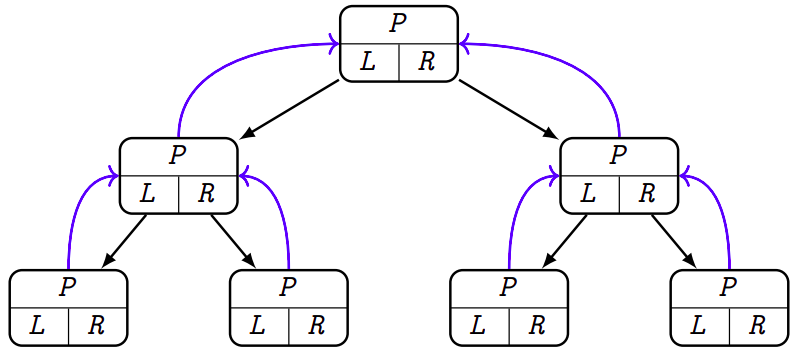
\includegraphics[width=0.7\textwidth]{memorizzazione-albero-binario.png}
    \caption{Schema di memorizzazione di un \emph{albero binario}}
\end{figure}

\subsection{Implementazione di un albero binario}
\begin{code}{Implementazione di un albero binario}
    \begin{minipage}[t]{0.48\textwidth}
        \ind Tree(\bc{ITEM} v)\\
            \bc{TREE} t = new \bc{TREE}\\
            t.parent = nil\\
            t.left = nil\\
            t.right = nil\\
            t.value = v\\
            return t\\
        
        \ind\bc{ITEM} read()\\
            return value\\

        \ind write(\bc{ITEM} v)\\
            value = v\\

        \ind\bc{TREE} parent()\\
            return parent\\

        \ind\bc{TREE} left()\\
            return left\\

        \ind\bc{TREE} right()\\
            return right\\
    \end{minipage}
    \hfill
    \begin{minipage}[t]{0.48\textwidth}
        \com{Ipotizziamo che sia possibile}
        \com{inserire un \emph{figlio} solo se non}
        \com{ne esiste già uno}
        \rmbreak\ind insertLeft(\bc{TREE} t)\\
            \indf if (left == nil) then\\
                t.parent = this\\
                left = t\\

        \ind insertRight(\bc{TREE} t)\\
            \indf if (right == nil) then\\
                t.parent = this\\
                right = t\\

        \ind deleteLeft()\\
            \indf if (left $\neq$ nil) then\\
                left.deleteLeft()\\
                left.deleteRight()\\
                delete left\\
                left = nil\\
            
        \ind deleteRight()\\
            \indf if (right $\neq$ nil) then\\
                right.deleteLeft()\\
                right.deleteRight()\\
                delete right\\
                right = nil\\
    \end{minipage}
\end{code}

\subsection{Visite di un albero binario}
\begin{definition}[Visita di un albero]
    Una visita è una strategia per visitare tutti i nodi dell'albero.
\end{definition}
\begin{definition}[Visita in profondità (depth first search)]
    Una visita in profondità è un tipo di visita nella quale vengono visitati
    ricorsivamente tutti i sottoalberi.
\end{definition}
\begin{note}
    Questo tipo di \emph{visita} richiede l'utilizzo di una \emph{pila}.
\end{note}\noindent
Per la \emph{visita in profondità} esistono tre varianti che si differenziano per
il momento in cui viene utilizzato il valore di un \emph{nodo}:
\begin{itemize}
    \item \emph{Visita in Pre-order}: il valore del \emph{nodo} viene usato prima
    di visitare i \emph{sottoalberi};
    \item \emph{Visita in In-order}: il valore del \emph{nodo} viene usato dopo
    aver visitato il \emph{sottoalbero di sinistra} e prima di visitare quello di
    \emph{destra};
    \item \emph{Visita in Post-order}: il valore del \emph{nodo} viene usato dopo
    aver visitato i \emph{sottoalberi}; 
\end{itemize}

\begin{definition}[Visita in ampiezza (breadth first search)]
    Una visita in ampiezza è un tipo di visita nella quale l'albero viene
    visitato un livello alla volta partendo dalla radice. 
\end{definition}
\begin{note}
    Questo tipo di \emph{visita} richiede l'utilizzo di una \emph{coda}.
\end{note}

\paragraph{Implementazione delle visite}
\begin{code}{Implementazione delle visite}
    \begin{minipage}[t]{0.48\textwidth}
        \com{Depth-First-Search in Pre-order}
        \rmbreak\ind dfs\_pre\_order(\bc{TREE} t)\\
            \indf if (t $\neq$ nil) then\\
                print t.value\\
                dfs\_pre\_order(t.left)\\
                dfs\_pre\_order(t.right)\\

        \noindent\com{Depth-First-Search in In-order}
        \rmbreak\ind dfs\_in\_order(\bc{TREE} t)\\
            \indf if (t $\neq$ nil) then\\
                dfs\_in\_order(t.left)\\
                print t.value\\
                dfs\_in\_order(t.right)\\

        \noindent\com{Depth-First-Search in Post-order}
        \rmbreak\ind dfs\_post\_order(\bc{TREE} t)\\
            \indf if (t $\neq$ nil) then\\
                dfs\_post\_order(t.left)\\
                dfs\_post\_order(t.right)\\
                print t.value\\
    \end{minipage}
    \hfill
    \begin{minipage}[t]{0.48\textwidth}
        \com{Breadth-First-Search}
        \rmbreak\ind bfs(\bc{TREE} t)\\
            \bc{QUEUE} q = Queue()\\
            q.enqueue(t)\\
            \indf while (not q.isEmpty()) do\\
                \bc{TREE} u = q.dequeue()\\
                print u.value\\
                \com{Accoda entrambi i \emph{figli}}
                \com{del \emph{nodo} corrente}
                u = u.left()\\
                \indff if (u $\neq$ nil) then\\
                    q.enqueue(u)\\
                
                \rmbreak\indf\\
                u = u.parent().right()\\
                \indff if (u $\neq$ nil) then\\
                    q.enqueue(u)\\
    \end{minipage}
\end{code}\noindent
\paragraph{Esempi di visite}\mbox{}\\
\begin{minipage}[t]{0.48\textwidth}
    Vediamo un esempio di utilizzo delle \emph{visite}:
    \begin{itemize}
        \item \emph{DFS Pre-order}: \texttt{A B C D E F G};
        \item \emph{DFS In-order}: \texttt{C B D A F E G};
        \item \emph{DFS Post-order}: \texttt{C D B F G E A};
        \item \emph{BFS}: \texttt{A B E C D F G};
    \end{itemize}
\end{minipage}
\hfill
\begin{minipage}[t]{0.48\textwidth}
    \begin{center}
        \begin{graph}
          \node[main] (0) {$A$};
          \node[main] (1) [below left of=0, xshift=-15] {$B$};
          \node[main] (2) [below right of=0, xshift=15] {$E$};
          \node[main] (3) [below left of=1, xshift=10] {$C$};
          \node[main] (4) [below right of=1, xshift=-10] {$D$};
          \node[main] (5) [below left of=2, xshift=10] {$F$};
          \node[main] (6) [below right of=2, xshift=-10] {$G$};
      
          \path[-]  (0) edge (1)
                    (0) edge (2)
                    (1) edge (3)
                    (1) edge (4)
                    (2) edge (5)
                    (2) edge (6);
        \end{graph}
      \end{center}
\end{minipage}

\begin{note}
    Il \emph{costo computazionale} di una \emph{visita} di un \emph{albero}
    contenente $n$ \emph{nodi} è $\Theta(n)$ poiché ogni \emph{nodo} viene
    visitato una sola volta.
\end{note}

\newpage
\section{Alberi generici}
Negli \emph{alberi generici}, ovviamente, non possiamo parlare di \emph{figlio
sinistro} e \emph{figlio destro}, ma possiamo comunque distinguere i \emph{figli}
di un \emph{nodo} in base alla loro posizione. Parleremo infatti, di
\emph{figlio più a sinistra}, o \emph{primo figlio}, e \emph{fratello destro},
o \emph{prossimo fratello}.

\subsection{Specifica}
\begin{code}{Albero generico}
    \com{Costituisce un nuovo \emph{nodo}, contenente $v$, senza \emph{figli} o
    \emph{genitori}}
    Tree(\bc{ITEM}  v)
    \nl\com{Legge il valore memorizzato nel \emph{nodo}}
    \bc{ITEM} read()
    \nl\com{Modifica il valore memorizzato nel \emph{nodo}}
    write(\bc{ITEM} v)
    \nl\com{Restituisce il \emph{padre}, oppure nil se questo è il \emph{nodo
    radice}}
    \bc{TREE} parent()
    \nl\com{Restituisce il primo \emph{figlio} da sinistra, oppure nil se
    questo \emph{nodo}}
    \com{è una \emph{foglia}}
    \bc{TREE} leftmostChild()
    \nl\com{Restituisce il primo \emph{fratello} sulla destra, oppure nil se
    è assente}
    \bc{TREE} rightSibling()
    \nl\com{Inserisce il \emph{sottoalbero} $t$ come primo \emph{figlio} di
    questo \emph{nodo}}
    insertChild(\bc{TREE} t)
    \nl\com{Inserisce il \emph{sottoalbero} $t$ come prossimo \emph{fratello} di
    questo \emph{nodo}}
    insertSibling(\bc{TREE} t)
    \nl\com{Distrugge l'\emph{albero radicato} identificato dal primo \emph{figlio}}
    deleteChild()
    \nl\com{Distrugge l'\emph{albero radicato} identificato dal prossimo \emph{fratello}}
    deleteSibling()
    \nl\com{Distrugge l'\emph{albero radicato} identificato dal \emph{nodo}}
    delete(\bc{TREE} t)
\end{code}

\subsection{Memorizzazione di un albero generico}
A differenza degli \emph{alberi binari}, per gli \emph{alberi generici} esistono
diversi modi per rappresentarli in memoria. I modi sono tre:
\begin{itemize}
    \item \emph{Vettore dei figli}: ogni \emph{nodo} contiene un riferimento al
    \emph{padre} e un vettore contenente i puntatori ai \emph{figli};
    \item \emph{Primo figlio, prossimo fratello}: ogni \emph{nodo} contiene un
    riferimento al \emph{padre} e un riferimento al prossimo \emph{fratello};
    \item \emph{Vettore dei padri}: l'\emph{albero} è rappresentato da un
    vettore di coppie nelle quali il primo valore è il valore associato al
    \emph{nodo} e il secondo è l'indice della posizione del \emph{padre} nel
    vettore;
\end{itemize}

\begin{note}
    L'approccio con \emph{vettore dei figli} può causare uno spreco di memoria
    se molte celle di quei vettori puntano a \texttt{nil}.
\end{note}
\paragraph{Tecniche di memorizzazione a confronto}\mbox{}\\
\begin{figure}[h!]
    \centering
    \subfloat[\emph{Vettore dei figli}]{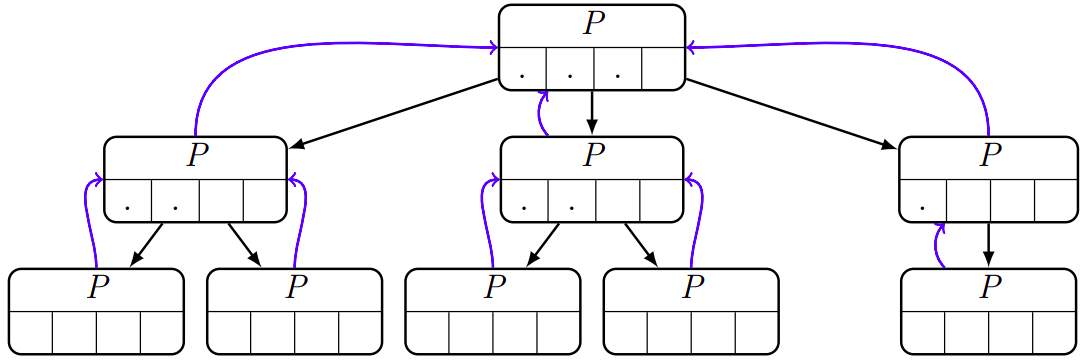
\includegraphics[width=0.48\textwidth]{vettore-dei-figli.png}}
    \hfill
    \subfloat[\emph{Primo figlio, prossimo fratello}]{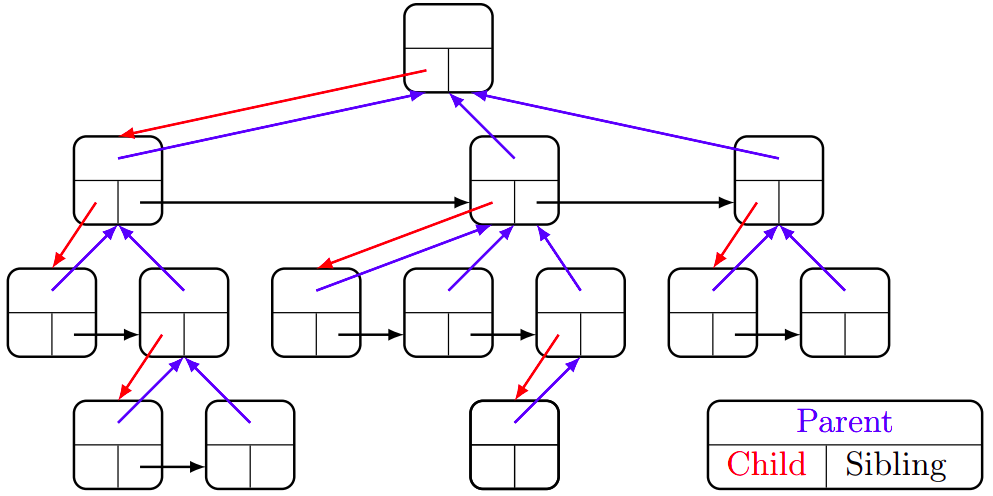
\includegraphics[width=0.48\textwidth]{vettore-dei-fratelli.png}}\\
    \subfloat[\emph{Vettore dei padri}]
    {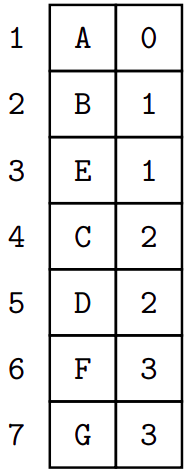
\includegraphics[width=0.1\textwidth, align=t]{vettore-dei-padri.png}
    \hspace{30pt}
    \begin{graph}
        \node[main] (0) [yshift=-15] {$A$};
        \node[main] (1) [below left of=0, xshift=-15] {$B$};
        \node[main] (2) [below right of=0, xshift=15] {$E$};
        \node[main] (3) [below left of=1, xshift=10] {$C$};
        \node[main] (4) [below right of=1, xshift=-10] {$D$};
        \node[main] (5) [below left of=2, xshift=10] {$F$};
        \node[main] (6) [below right of=2, xshift=-10] {$G$};
    
        \path[-]  (0) edge (1)
                  (0) edge (2)
                  (1) edge (3)
                  (1) edge (4)
                  (2) edge (5)
                  (2) edge (6);
    \end{graph}}
    \caption{Memorizzazione di \emph{alberi generici}}
\end{figure}

\subsection{Implementazione di un albero generico}
Di seguito, è riportata l'implementazione di un \emph{albero generico} realizzato
con la tecnica di memorizzazione \emph{primo figlio, prossimo fratello}.

\begin{code}{Implementazione di un albero generico}
    \begin{minipage}[t]{0.48\textwidth}
        \bc{TREE} parent\hfill\com{Riferimento al \emph{padre}}
        \bc{TREE} child\hfill\com{Riferimento al}
        \mbox{}\hfill\com{primo \emph{figlio}}
        \bc{TREE} sibling\hfill\com{Riferimento al}
        \mbox{}\hfill\com{prossimo \emph{fratello}}
        \bc{ITEM} value\hfill\com{Valore}

        \ind\bc{TREE} Tree(\bc{ITEM} v)\\
            \bc{TREE} t = new \bc{TREE}\\
            t.value = v\\
            t.parent = nil\\
            t.child = nil\\
            t.sibling = nil\\
            return t
    \end{minipage}
    \hfill
    \begin{minipage}[t]{0.48\textwidth}
        \vspace{-8.5pt}
        \com{Inserisce $t$ prima dell'attuale}
        \com{\emph{figlio}}
        \rmbreak\ind insertChild(\bc{TREE} t)\\
            t.parent = this\\
            t.sibling = child\\
            child = t\\
        
        \com{Inserisce $t$ prima dell'attuale}
        \com{prossimo \emph{fratello}}
        \rmbreak\ind insertSibling(\bc{TREE} t)\\
                t.parent = parent\\
                t.sibling = sibling\\
                sibling = t\\
    \end{minipage}
\end{code}
\begin{codecont}
    \begin{minipage}[t]{0.48\textwidth}
        \ind\bc{ITEM} read()\\
            return value\\

        \ind write(\bc{ITEM} v)\\
            value = v\\

        \ind\bc{TREE} parent()\\
            return parent\\
            
        \ind\bc{TREE} leftmostChild()\\
            return child\\

        \ind\bc{TREE} rightSibling()\\
            return sibling\\
    \end{minipage}
    \hfill
    \begin{minipage}[t]{0.48\textwidth}
        \ind deleteChild()\\
            \bc{TREE} c = child.rightSibling()\\
            delete(child)\\
            child = c\\

        \ind deleteSibling()\\
            \bc{TREE} s = sibling.rightSibling()\\
            delete(sibling)\\
            sibling = s\\

        \ind delete(\bc{TREE} t)\\
            \bc{TREE} u = t.leftmostChild()\\
            \indf while (u $\neq$ nil) do\\
                \bc{TREE} next = u.rightSibling()\\
                delete(u)\\
                u = next\\
            \indf delete t\\
    \end{minipage}
\end{codecont}

\subsection{Visite di un albero generico}
Anche per gli \emph{alberi generici} valgono le stesse \emph{visite} viste
per gli \emph{alberi binari} ad eccezione della \emph{visita In-order} perché
in questo caso non è ben definibile una situazione intermedia.

\paragraph{Implementazione delle visite}
\begin{code}{Implementazione delle visite}
    \begin{minipage}[t]{0.48\textwidth}
        \com{Depth-First-Search in Pre-order}
        \rmbreak\ind dfs\_pre\_order(\bc{TREE} t)\\
            \indf if (t $\neq$ nil) then\\
                print t.value\\
                \bc{TREE} u = t.leftmostChild()\\
                \indff while (u $\neq$ nil) do
                    dfs\_pre\_order(u)\\
                    u = u.rightSibling()\\

        \noindent\com{Depth-First-Search in Post-order}
        \rmbreak\ind dfs\_post\_order(\bc{TREE} t)\\
            \indf if (t $\neq$ nil) then\\
                \bc{TREE} u = t.leftmostChild()\\
                \indff while (u $\neq$ nil) do
                    dfs\_post\_order(u)\\
                    u = u.rightSibling()\\
                \indff print t.value\\
    \end{minipage}
    \hfill
    \begin{minipage}[t]{0.48\textwidth}
        \com{Breadth-First-Search}
        \rmbreak\ind bfs(\bc{TREE} t)\\
            \bc{QUEUE} q = Queue()\\
            q.enqueue(t)\\
            \indf while (not q.isEmpty()) do\\
                \bc{TREE} u = q.dequeue()\\
                print u.value\\
                \com{Accoda tutti i \emph{figli}}
                \com{del \emph{nodo} corrente}
                u = u.leftmostChild()\\
                \indff while (u $\neq$ nil) do\\
                    q.enqueue(u)\\
                    u = u.rightSibling()\\
    \end{minipage}
\end{code}